\addcontentsline{toc}{chapter}{Оптимизация конструкции робота}

\textbf{\underline{Вторая глава}} показывает решения оптимизационных задач.

\textbf{Первая задача:} решить задачу оптимизации $F=f(x) \rightarrow max$, где  $f(x)$ --- критерии: пройденная дистанция, длина корпуса, $(x)$ --- параметры: количество ног, сдвиг фазы между соседними ногами \pic{fig:opti_criteria}. Количество ног имеет прямую зависимость с длиной корпуса робота. 

\begin{figure}[h]
    \begin{subfigure}{0.49\textwidth}
        \centering\includegraphics[height=2cm,width=1\textwidth,keepaspectratio]{f1.png}
        \caption{Кол-во ног $\uparrow$, детализация поверхности $\uparrow$}
        \label{fig:f1.png}
    \end{subfigure}
    \begin{subfigure}{0.49\textwidth}
        \centering\includegraphics[height=1.5cm,width=1\textwidth,keepaspectratio]{f2.png}
        \caption{Длина робота $\uparrow$, курсовая проходимость $\downarrow$}
        \label{fig:f2.png}
    \end{subfigure}

    \hfill
    \begin{subfigure}{\textwidth}
        \centering\includegraphics[height=1.5cm,width=1\textwidth,keepaspectratio]{f3_new.png}
        \caption{Длина робота $\uparrow$, профильная проходимость $\uparrow$}
        \label{fig:f3.png}
    \end{subfigure}
    \hfill

\caption{Критерии оптимизации конструкции робота}
\label{fig:opti_criteria}
\end{figure}

В основе метода лежит генетический алгоритм Open AI-ES. Метод работает следующим образом: генерируется множество особей, а также семейство территорий с одинаковой сложностью \pic{fig:terrains}. За фиксированное время, с постоянной угловой скоростью на моторах, каждый робот проходит это семейство территорий и записываются данные. Делаются следующие предположения: есть только сухое трение между ногами и поверхностью, созданные поверхностью с помощью одной функции и параметров имеют одинаковую сложность. Целевая функция \eqref{eq:second}.

\begin{align}
    \label{eq:second}
    F \rightarrow max = \beta \left( {\omega}_{1} \cdot \delta + {\omega}_{2} \cdot L\right) + (1 - \beta) {\delta}^{{\omega}_{1}} {\left( L\right)}^{{\omega}_{2}} \\
    L = \frac{1}{(\gamma - 1) h_{\text{leg}}sin(\alpha)}
\end{align}
Где $\beta$ -- адаптивный параметр, ${\omega}_{1,2} \in  [ 0..1 ],\ \omega_1 + \omega_2 = 1 $ -- весовые коэффициенты, $\delta$ -- пройденный путь, $L$ -- упрощенная длина робота. Количество движителей по каждому из бортов обозначается через $\gamma$. Разность фаз между соседними движителями обозначается через $\alpha$ \pic{fig:best_gen_robot.jpg}.

\begin{figure}[h]
    \begin{subfigure}{0.33\textwidth}
    \centering\includegraphics[width=0.8\textwidth]{terrain_1} 
    \caption{T1: 3D-боксы с равномерным распределением высоты}
    \label{fig:terrain_1}
    \end{subfigure}
    \begin{subfigure}{0.33\textwidth}
    \centering\includegraphics[width=0.8\textwidth]{terrain_2} 
    \caption{T2: 2D-полосы с гауссовой функциональной высотой}
    \label{fig:terrain_2}
    \end{subfigure}
    \begin{subfigure}{0.33\textwidth}
    \centering\includegraphics[width=0.8\textwidth]{terrain_3}
    \caption{T3: 2D-полосы с распределением высоты по гауссовой функции)}
    \label{fig:terrain_3}
    \end{subfigure}
     
    \caption{Примеры сгенерированных территорий}
    \label{fig:terrains}
\end{figure}


\begin{figure}[h]
    \begin{subfigure}[t]{0.59\textwidth}
        \centering\includegraphics[height=3cm,width=1\textwidth,keepaspectratio]{robot_scheme_optim.png}
        \caption{Схема модели робота для генетического алгоритма}
        \label{fig:best_gen_robot.jpg}
    \end{subfigure}
    \begin{subfigure}[t]{0.39\textwidth}
        \centering\includegraphics[height=4cm,width=1\textwidth,keepaspectratio]{images/Strirus_leg.drawio.png}
        \caption{Отображение переменных для модели взаимодействия опорной поверхности и ноги робота}
        \label{fig:contact_interaction.png}
    \end{subfigure}

\caption{Пример модели робота}
\end{figure}

\textit{Описание математической модели}. Робот представляет собой механическую систему, состоящую из твердых тел \eqref{eq:newton_euler}. Движение которых описывается дифференциальными уравнениями вида:

\begin{align}
    \label{eq:newton_euler}
    M \dot{\vec{u}} = \vec{g} \\
% \end{align}
% \begin{align}
    M = \begin{bmatrix}
    M_1 & \cdots  & 0 \\
    \vdots  & \ddots  & \vdots  \\ 
    0 & \cdots   & M_n 
    \end{bmatrix},\ M_i = \begin{bmatrix}
    m_i E_{3\times 3} & 0 \\ 
    0 & I_i 
    \end{bmatrix} \\
% \end{align}
% \begin{align}
    \vec{u}_i^{\ T} = \begin{bmatrix}
        \vec{v}_i^{\ T} & \vec{\omega}_i^{\ T}
    \end{bmatrix} \\ 
    \vec{g}^{\ T} = \begin{bmatrix}
        \cdots \  \vec{F}_i^{\ T}, & (\vec{\tau}_i - \vec{\omega}_i \times I_i \vec{\omega}_i)^T\  \cdots 
    \end{bmatrix}
\end{align}
где, $M_i$ --- матрицы, содержащие массово-инерционные характеристики; $m_i$ масса тела; $I_i$ тензор инерции; $\vec{u_i}$ вектор обобщённых скоростей; $E$ --- единичная матрица; $\vec{g}$ вектор обобщённых сил; $\vec{v_i}$ вектор линейной скорости; $\vec{\omega_i}$ --- вектор угловой скорости; $\vec{F_i}$, $\vec{\tau_i}$ силы и моменты сил взаимодействия.

Тела, входящие в систему соединены между собой цилиндрическими шарнирами, которые описываются следующими связями и динамическими ограничениями \eqref{eq:kin_constr}:
\begin{align}
    \label{eq:kin_constr}
    \phi(q_{j_1},\ \cdots,\ q_{j_k},\ t) \geqslant  0 \\
    \vec{q_i}^{\ T} = \begin{bmatrix}
        \vec{x}_i^{\ T} & \vec{Q}_i^{\ T}
    \end{bmatrix} \\
    \dot{\vec{q_i}} = \begin{bmatrix}
    E_{3\times3} & 0\\ 
    0 & G(\vec{q}_i) 
    \end{bmatrix}\vec{u}_i  \\
    \vec{g}_i = \tau_i^T \vec{z}_{i-1} -k_i \dot{\vec{q_i}}
\end{align}
где через $\phi$ обозначена функция связи; $t$ время; $q_{j}$ --- вектор обобщенных координат, включающий в себя координаты центра масс $\vec{x_i}$ и кватернион $\vec{Q_i}$, описывающий ориентацию тела в пространстве; через $G(\vec{q}_i)$ обозначена матрица, вид которой зависит от выбранной системы координат и способа задания ориентации тела; $k$~---~ коэффициент вязкого трения в шарнире.

Контакт ног робота с опорной поверхностью \pic{fig:contact_interaction.png} описывается на базе модели сухого трения и выражается следующими уравнениями \eqref{eq:contact_inter}:

\begin{align}
    \label{eq:contact_inter}
    \phi_u(\vec{q}\ ) \geqslant 0 \\ 
                        \phi_u(\vec{q}\ ) = (\vec{x}_1 + \vec{s}_1 - \vec{x}_2 - \vec{s}_2) \cdot \vec{n} \\
                        \frac{d }{d t}\phi_u(\vec{q}\ ) \approx \begin{bmatrix}
                            \vec{n}^{\ T} & (\vec{s}_1 \times \vec{n})^T & -\vec{n}^{\ T} & (-\vec{s}_2 \times \vec{n})^T
                        \end{bmatrix} \begin{bmatrix}
                            \vec{v}_1\\ 
                        \vec{\omega}_1\\ 
                        \vec{v}_2\\
                        \vec{\omega}_2\\
                        \end{bmatrix} \\
\left\{\begin{matrix*}[l]
\mu f_n \geqslant \sqrt{f_1^2 + f_2^2}\\ 
\left\lVert \vec{v_t}\right\rVert (\mu f_n - \sqrt{f_1^2 + f_2^2}) = 0\\
\dfrac{\vec{f_t}}{\left\lVert \vec{f_t}\right\rVert } = - \dfrac{\vec{v_t}}{\left\lVert \vec{v_t}\right\rVert }
\end{matrix*}\right.
\end{align}
где, $\phi_u(\vec{q})$ --- функция связи; $\mu $ --- коэффициент трения между ногой и опорной поверхностью; $\vec{x}_{1,2},\ \vec{s}_{1,2}$ --- радиус-векторы и орты координатных осей $\vec{t}_{1,2}, \vec{n}$ показаны на рисунке \pic{fig:contact_interaction.png}; $ f_{1,2} $ --- значения сил трения вдоль осей $t_{1,2}$.

% Численные эксперименты выполнялись в симуляторе Gazebo. В качестве примера видеозапись одного из экспериментов можно посмотреть по ссылке в QR-коде \quad \qrcode[height=1.5cm]{https://youtu.be/DcovvkTZgsg}

Одним из основных результатов исследования, полученных при варьировании значений весовых коэффициентов $\omega$ является зависимость между количеством ног и пройденной дистанцией, которая показала наличие локального оптимума при количестве ног у робота в диапазоне от 8 до 14. 

% \begin{figure}[H]
%     \centering\includegraphics[height=5cm,width=1\textwidth,keepaspectratio]{images/box_plot_structural_synthesis.png}
%     \caption{Зависимость между количеством ног и пройденной дистанцией}
%     \label{fig:box_plot_structural_synthesis.png}
% \end{figure}

\textbf{Вторая задача:} разработать концепт корпуса робота для максимизации курсовой проходимости, без изменения длины ног робота.

\begin{figure}[h]
    \centering\includegraphics[height=4cm,width=1\textwidth,keepaspectratio]{vector_representation_rus.png}
    \caption{Векторное представление сил в классическом и всенаправленном вариантах робота}
    \label{fig:omnidirection}
\end{figure}

На рисунке \ref{fig:omnidirection} представлена иллюстрация данной концепции: для того, чтобы робот двигался во всех направлениях, необходимо разделить ноги на группы, чтобы получилось 4 группы A-D и сделать так, чтобы угол между корпусом робота и осью вала привода ноги не был равен 90 градусам. 

Стрелка в центре робота --- результирующая всех сил. Если изменить угол оси привода ноги в соответствии с предлагаемой концепцией, к примеру при этапе проектирования, то возможно получить вектор результирующей силы, представленный на рис. \ref{fig:omnidirection} в центре. Для того, чтобы переместить корпус робота вправо, группы A и D должны вращать ногу в одну сторону, а группы C и B --- в противоположную.

% Возможности, полученные с помощью оптимизации конструкции робота можно посмотреть по ссылке в QR-коде \quad \qrcode[height=1.5cm]{https://youtu.be/EQ6oGZVDpoc}

Результатом главы стал метод, который позволяет оптимизировать конструкцию класса многоногих шагающих роботов с цельным или сочленённым корпусом, и цикловыми движителями с одной степенью свободы, управляемые зависимо или независимо друг от друга для решения задачи определения геометрических и физико-механических свойств пройденной поверхности.

